\newpage
\section{Логарифмический вычет, его вычисление. Приращение (полярного) аргумента вдоль пути. Принцип аргумента. Теорема Руше и ее применение.}

Пусть $f \in H(\mathring{U_r}(a)), a \in \mathbb{C}, r > 0$. Тогда вычет функции $\frac{f'(z)}{f(z)} = \frac{d}{dt}Lnf(z)$ в точке $a$ называют \textbf{логарифмическим вычетом функции $f$ в точке $a$.}\\[2mm]

\textbf{Лемма о логарифмическом вычете в нуле и в полюсе:}\\[2mm]
Логарифмический вычет ф. $f(z)$ в точке $a$ равен:
\begin{enumerate}
    \item порядку нуля $a$, если $a$ -- нуль
    \item пордяку полюса $a$, если $a$ -- полюс
\end{enumerate}

\begin{proof}
    \ \\
    1) Пусть $a$ --- нуль порядка $n$ ф-ии $f(z)$, тогда:\\
    $f(z) =a_n(z-z)^n + a_{n+1}(z-a)^{n+1}+...=(z-a)^n\cdot \varphi(z)$, где
    $\varphi(z)$ --- сумма степенного ряда, откуда следует, что $\varphi \in H$\\[2mm]
    $\varphi(z)=c_n\neq0\Rightarrow \frac{f'(z)}{f(z)}=\frac{n(z-a)^{n-1}\cdot \varphi(z)+(z-a)^{n}\varphi'(z)}{(z-a)^n \varphi(z)}=\frac{1}{z-a}(n+(z-a)\cdot \frac{\varphi'(z)}{\varphi(z)}) \Rightarrow a$ --- полюс 1-ого порядка функции $\frac{f'}{f} \Rightarrow C_{-1}=n$, т.к. $\frac{n}{z-a}$ --- главная часть.\\[2mm]
    2) Пусть $a$ --- полюс порядка $p$, тогда по теорему о полюсе $a$ --- нуль порядка $p$ функции $\frac{1}{f(z)}=g(z)$.\\
    $\frac{f'(z)}{f(z)} = -\frac{d}{dz} Ln\frac{1}{f(z)}$\\
    Тогда логарифмический вычет функции $g$ в точке $a$ равен $p$, а функции $f$ в точке $a$ равен $-p$.
\end{proof}
\ \\

\textbf{Теорема о логарифмическом вычете:}\\[2mm]
Пусть $f$ мероморфна в области $D \subset \mathbb{C}, G \cup \partial G \subset D, \partial G$ не содержит ни нулей, ни полюсов функции $f$, $N$ и $P$ -- количество нулей и полюсов с учетом их порядков функции $f$ в $G$.\\
Тогда $\frac{1}{2\pi i}$ \(\int\limits_{\partial G} \frac{f'(z)}{f(z)}\, dz\) $= N - P$ (обход $\partial G$ против часовой стрелки),\\
где \(\int\limits_{\partial G} \frac{f'(z)}{f(z)}\, dz\) -- логарифмический вычет функции $f$ вдоль кривой $\partial G$.

\begin{proof}
    \ \\
    Особые точки $\frac{f'(z)}{f(z)}$ в области $G$:
    \begin{enumerate}
        \item полюса $a_1, .., a_l$ с порядками $p_1, ..., p_l$
        \item нули $b_1, .., b_m$ с порядками $n_1, ..., n_m$
    \end{enumerate}
    Тогда по лемме о логарифмическом вычете $\frac{f'}{f}(a_j)=-p_j$, $res\frac{f'}{f}(b_s)=n_s$\\
    По теореме Коши:
    $$\frac{1}{2\pi i}\int\limits_{\partial G} \frac{f'(z)}{f(z)}dz =\frac{1}{2\pi i}\cdot 2\pi i \left(\sum_{j=1}^l res\frac{f'}{f} (a_j) + \sum_{s=1}^m res \frac{f'}{f)}(b_s)\right) =$$
    $$= - \sum_{j=1}^l p_j +\sum_{s=1}^m n_s = N-P$$
\end{proof}


$\Delta_{\gamma}arg f = 2\pi k$, k -- количество обходов точки О f(z), $z \in \gamma$, с учетом приращения.

\begin{figure}[h]
    \centering
    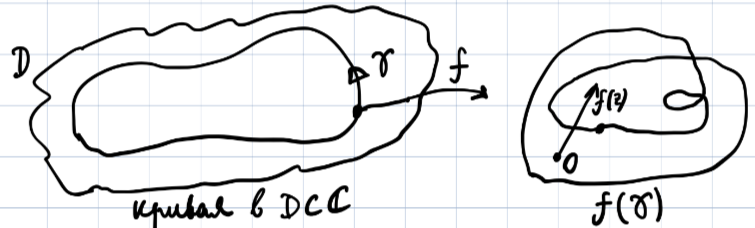
\includegraphics[width=0.5\linewidth]{answers/img/image1.png}
    \label{fig:enter-label}
\end{figure}

\textbf{Принцип аргумента}. Пусть f мераморфна в $ D \subset \mathbb{C}, \, G \cup \partial G \subset D, \, \partial G$ не содержит ни нулей, ни полюсов f. Тогда 

$N-P = \frac{1}{2 \pi}\Delta_{\partial G}arg f$.

\begin{proof}
    \ \\
    Пусть $\partial G: \ z=z(t), \ t\in[\alpha, \beta]$,
    $\Phi(t)=\ln f(z(t))$, где $\ln f$ непрерывно меняется при росте $t$ от $\alpha$ до $\beta$. Тогда $\Phi'(t)=\frac{f'(z(t))}{f(z(t))}\cdot z'(t)$ и поэтомy
    $$\int\limits_{\partial G}\frac{f'}{f}dz = \int\limits_{\alpha}^{beta} \frac{f'(z(t))}{f(z(t))}z'(t)dt=\Phi(\beta) - \Phi(\alpha) = $$
    $$= \ln f(z(\beta))-\ln f(z(\alpha)) = \ln |f(z(\beta))| + i \, arg \, f(z(\beta))-\ln |f(z(\alpha))|-$$
    $$= -i\cdot arg\, f(z(\alpha))=i\Delta_{\partial G}arg \, f = \text{ (по т. о логар.выч.) }N-P=$$
    $$=\frac{1}{2\pi i}\int\limits{\partial G} \frac{f'(z)}{f(z)}dt=\frac{i\Delta_{\partial G}arg\,f}{2\pi i}$$
\end{proof}


\textbf{Теорема Руше:}\\
Пусть $f,g \in H(G \cup \partial G) \, \textrm{и} \, \forall z \in \partial G |f(z)| > |g(z)|$. \\
Тогда функции f и f+g имеют одинаковое количество нулей в G.\\[2mm]

\begin{proof}
    \ \\
    $\forall z \in \gamma G |f(z)|>|g(z)|\geq 0$\\
    $|(f+g)(z)|\geq |f(z)|-|g(z)| > 0$\\
    Отсюда следует, что функция $f$ и $f+g$ не имеют нулей на $\partial G$.\\
    По принципу аргумента $\Delta_{\partial G}arg\, (f+g) = N_{f+g}$ (количество нулей функции $f+g$ в $G$).\\
    С другой стороны:\\
    $\Delta \gamma G arg\, f(1+\frac{g}{f})=\Delta_{\gamma G} arg\, f+\Delta_{\gamma G}(1+\frac{g}{f})=N_f$\\
    
\end{proof}
\textbf{Применение:}\\
Найти число корней уравнения $z^8-4z^5+z^2-1=0$ в области $|z|<1$.\\
На границе области $|z|=1$, тогда т.к. $|z^8+z^2-1|\leq |z|^8+|z|^2+|-1|=3 < |-4z^5|=4$ и уравнение $-4z^5=0$ имеет 5 корней в этой области, то исходное уравнение также иммеет 5 корней в этой области.